% !TeX root = 高等微积分.tex

\begin{definition}
    称$X$的子集$B$为上述拓扑$\left( X,\mathscr{T} \right) $的闭集(close set), 若$X / B = B^{C}$是开集.
\end{definition}

前面我们已经知道, 一个度量$d$可以诱导出一个度量拓扑$\mathscr{T}_{d}$, \textbf{在微积分中, 我们都是用此拓扑.}
\begin{itemize}
    \item 一元微积分中 $X = \mathbb{R}$, $d \left( x,y \right)  = \left| x -  y \right|$. $\mathbb{R}$上赋予欧式拓扑, 开集可以表示为一族开区间之并.
    
    \item 多元微积分中 $X = \mathbb{R}^{n}$, $d\left( \vec{x},\vec{y} \right)  = \sqrt{\sum \left( x_i  - y_i \right) ^{2}}$. $\mathbb{R}^{n}$上赋予欧式拓扑, 开集可以表示为一族不带边球体之并.
\end{itemize}

\begin{definition}
    设$\left( X, \mathscr{T} \right) $是一个拓扑空间, 给定$Y \subseteq X$, 令
    \begin{equation}
      \mathscr{T}_{Y} = \{ U \cap Y | U \in \mathscr{T} \}.
    \end{equation}
\end{definition}
易验证$\mathscr{T}_{Y}$是$Y$上的一个拓扑, $Y$(从$X$获得的)子空间拓扑.

我们以后对于$D \subseteq RT^{n}$, 都赋予从$\mathbb{R}^{n}$获得的子空间拓扑.

\begin{example}
    对于$D = [a,b] \subseteq  \mathbb{R}$, 它当中的开集可以为$[a,p) \cup (c,d) \cup (q,b]$
\end{example}

\subsubsection{基本概念}
\begin{definition}
    设$\left( X, \mathscr{T} \right) $是拓扑空间, 设$A \subseteq X, a \in A$.
    
    称$a$是$A$的内点(同时称$A$是$a$的邻域), 如果存在开集$U$, 使得$a \in U \subseteq A$.
\end{definition}

\begin{proposition}
    $A$是$X$的开集, 当且仅当$A$中每一点都是$A$的内点.
\end{proposition}

\begin{proof}
    从充分性和必要性两方面.

    \textbf{``$\implies$:''} 显然. $\forall a \in A$, 取开集$U = A$, 则$a \in U \subseteq  A$.

    \textbf{``$\impliedby$:''} 设$A$中每一点都是$A$的内点, 则$\forall a \in A$, $\exists U_a \in A$, $a \in U_a \subseteq A$. 则
    \begin{equation}
      A = \bigcup_{a \in A} \{ a \} \subseteq \bigcup_{a \in A} U_a \subseteq A.
    \end{equation}
    因而$A$是开集之并, 由拓扑公理三, $A$是开集.
\end{proof}

对于$\mathbb{R}^{n}$中的拓扑, $A$是$\mathbb{R}^{n}$的开集 $\iff$ $\forall a \in A$, $\exists B_{r}\left( a \right) \subseteq A$.

$B$是$\mathbb{R}^{n}$的闭集 $\iff$ $B^{C}$是$\mathbb{R}^{n}$的开集 $\iff$ $\forall y \notin B$, $\exists B_{r}\left( y \right) \subseteq  B^{C}$.

\subsubsection{连续性}
\begin{definition}
    设$\left( X, \mathscr{T}_{X} \right) $, $\left( Y, \mathscr{T}_{Y} \right) $是两个拓扑空间. 设$f\colon X \to Y$是一个映射, $x_0 \in X$. 
    
    称$f$在$x_0$处连续, 如果对于$Y$中任意开集$V \ni f\left( x_0 \right) $都存在$X$的开集$U \ni x_0$, 使$f\left( U \right) \subseteq V$.
\end{definition}

\begin{definition}
    称$f\colon X \to Y$为连续映射(记为$f \in C \left( X , Y \right) $), 如果$f$在$X$的每一点处都连续.
\end{definition}

\begin{theorem}
    $f\colon X \to Y$连续 
    
    $\iff$ $f$ 下开集的原像集是开集 (即对$Y$的任何开集$V$有$f^{-1} \left( V \right) $是$X$的开集).
    \footnote{注意这里面的$f^{-1}$并不是逆映射, 而是原像集
    \begin{equation}
        f^{-1} \left( V \right)  = \{ x \in X | f\left( x \right) \in V \}.
    \end{equation}
    }
    
    $\iff$ $f$下闭集的原像集是闭集 (对$Y$的任何闭集$B$有$f^{-1}\left( B \right) $是$X$的闭集).
\end{theorem}



\tikzset{every picture/.style={line width=0.75pt}} %set default line width to 0.75pt        

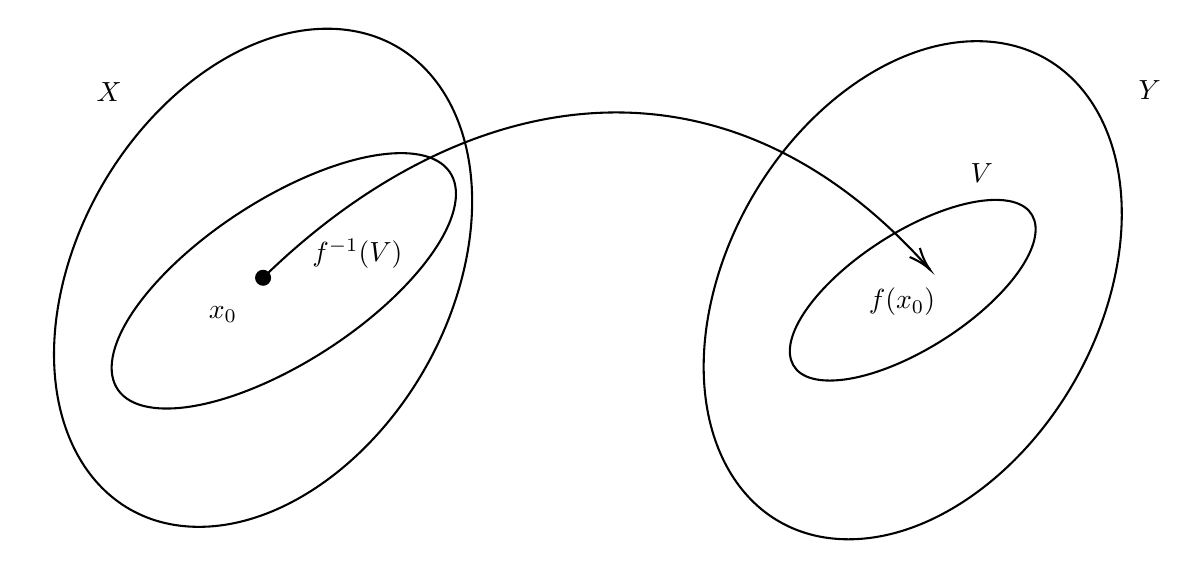
\begin{tikzpicture}[x=0.75pt,y=0.75pt,yscale=-1,xscale=1]
%uncomment if require: \path (0,300); %set diagram left start at 0, and has height of 300

%Shape: Ellipse [id:dp6956114134793403] 
\draw   (75.8,126.9) .. controls (92.88,60.63) and (149.63,6.9) .. (202.56,6.9) .. controls (255.49,6.9) and (284.55,60.63) .. (267.47,126.9) .. controls (250.4,193.17) and (193.64,246.9) .. (140.71,246.9) .. controls (87.79,246.9) and (58.72,193.17) .. (75.8,126.9) -- cycle ;
%Shape: Ellipse [id:dp4169675177352954] 
\draw   (388.8,132.9) .. controls (405.88,66.63) and (462.63,12.9) .. (515.56,12.9) .. controls (568.49,12.9) and (597.55,66.63) .. (580.47,132.9) .. controls (563.4,199.17) and (506.64,252.9) .. (453.71,252.9) .. controls (400.79,252.9) and (371.72,199.17) .. (388.8,132.9) -- cycle ;
%Shape: Ellipse [id:dp8474608971788034] 
\draw   (120.88,128.37) .. controls (152.09,94.4) and (204.57,66.85) .. (238.12,66.85) .. controls (271.66,66.85) and (273.56,94.4) .. (242.36,128.37) .. controls (211.16,162.35) and (158.67,189.9) .. (125.13,189.9) .. controls (91.58,189.9) and (89.68,162.35) .. (120.88,128.37) -- cycle ;
%Shape: Ellipse [id:dp07298221921958703] 
\draw   (440.94,132.9) .. controls (463.02,108.86) and (500.47,89.37) .. (524.6,89.37) .. controls (548.74,89.37) and (550.4,108.86) .. (528.33,132.9) .. controls (506.26,156.94) and (468.8,176.42) .. (444.67,176.42) .. controls (420.54,176.42) and (418.87,156.94) .. (440.94,132.9) -- cycle ;
%Curve Lines [id:da21482947459601198] 
\draw    (171.64,126.9) .. controls (265.87,34.9) and (391.87,8.9) .. (492.87,122.9) ;
\draw [shift={(492.87,122.9)}, rotate = 228.46] [color={rgb, 255:red, 0; green, 0; blue, 0 }  ][line width=0.75]    (10.93,-3.29) .. controls (6.95,-1.4) and (3.31,-0.3) .. (0,0) .. controls (3.31,0.3) and (6.95,1.4) .. (10.93,3.29)   ;
\draw [shift={(171.64,126.9)}, rotate = 315.69] [color={rgb, 255:red, 0; green, 0; blue, 0 }  ][fill={rgb, 255:red, 0; green, 0; blue, 0 }  ][line width=0.75]      (0, 0) circle [x radius= 3.35, y radius= 3.35]   ;

% Text Node
\draw (144,139.4) node [anchor=north west][inner sep=0.75pt]    {$x_{0}$};
% Text Node
\draw (90,31.4) node [anchor=north west][inner sep=0.75pt]    {$X$};
% Text Node
\draw (193.88,106.77) node [anchor=north west][inner sep=0.75pt]    {$f^{-1}( V)$};
% Text Node
\draw (462,130.4) node [anchor=north west][inner sep=0.75pt]    {$f( x_{0})$};
% Text Node
\draw (511,70.4) node [anchor=north west][inner sep=0.75pt]    {$V$};
% Text Node
\draw (592,30.4) node [anchor=north west][inner sep=0.75pt]    {$Y$};


\end{tikzpicture}


第一条推第二条: 
\begin{proof}[第一条推出第二条]
    设 $f \in C(X,Y )$ ,设 $V $ 是 $Y $ 中的开集,来证: $f^{-1}(V)$ 是 $X $ 的开集。\\
    这等价于证明, $f ^{-1} (V)$ 中的每点 $x_0$是 $f^{-1}(V)$ 的内点。\\
    由 $x_0 \in f^{-1}(V)$,知 $f(x_0) \in V$,由 $f $ 在 $x_0$ 处连续,知存在 $X$ 中的开集 $U$,使 $x_0 \in U$,且 $f(U) \subseteq V$。\\  
    即 $U \subseteq f^{-1}(V)$,这样,$x_0 \in U_{\text{(开)}} \subseteq f^{-1}(V)$,说明 $x_0$ 是 $f^{-1}(V)$ 的内点。\\
    又因为 $x_0$ 是 $f^{-1}(V)$ 中任意点,所以 $f^{-1}(V)$ 是开集。
\end{proof}


% 
% 
% 
% ========= 补充 ==========
% 
% 
% 
% 
\begin{proof}[第二条推出第一条]
    设$f$下开集的原像集都为开集, 来证$f \in C\left( X,Y \right) $, 即证$f$在每一点$x_0$处连续. 
    
    为此, 对任何开集$V \ni f\left( x_0 \right) $, 由于第二条成立可知 $f^{-1}\left( V \right) $是$X$的开集, 取$U = f^{-1} \left( V \right)$显然$x_0 \in f^{-1} \left( V \right)  = U$.
\end{proof}

\begin{proof}[证明第二条等价于第三条]
    假设$B$是一个闭集, 则$B^{C}$是一个开集, 由第二条可知$f^{-1} \left( B^{C} \right) $是一个开集. 注意到
    \begin{equation}
      X = f^{-1} \left( B \right) \sqcup f^{-1} \left( B^{C} \right) .
    \end{equation}
    即$ f^{-1} \left( B^{C} \right) = \left( f^{-1} \left( B \right)  \right) ^{C}$,
    所以$f^{-1} \left( B \right) $是一个闭集.
\end{proof}

\begin{theorem}[连续映射的复合是连续的]
    设$f \colon X \to Y$在$x_0$处连续, $g \colon Y \to Z$在$f\left( x_0 \right) $处连续.
    
    则$g \circ f \colon X \to Z$在$x_0$处连续.
\end{theorem}
\begin{proof}
    对任何包含$g \circ f\left( x_0 \right) $的任何开集$W$, 由 $g$在$f\left( x_0 \right) $处连续的定义, 存在含$f\left( x_0 \right) $的开集$V$是$g\left( V  \right) \subseteq W$.

    又由于$f$在$x_0$处连续的定义知, 存在含$x_0$的开集$U$使得$f\left( U \right) \subseteq V$.

    这样, $g \circ f \left( U \right) = g\left( f\left( U \right)  \right) \subseteq g\left( V \right) \subseteq W$. 从而$g \circ f$在$x_0$处连续.
\end{proof}

\begin{theorem}[映射复合保持连续性]
    设$f \in C\left( X,Y \right) $, $g \in C\left( Y,Z \right) $则 $g \circ f \in C\left( X, Z \right) $.
\end{theorem}
\begin{proof}[证法一]
    用定理的逐点版本来证.
\end{proof}
\begin{proof}[证法二]
    % 
    % 
    % 
    % ========= 补充 ===========
    % 
    % 
    % 
    % 
\end{proof}

前述定理是连续映射的局部性质, 下面我们讨论连续函数的局部性质.
\begin{theorem}
    设$f \colon X\to \mathbb{R}$, $g \colon X\to \mathbb{R}$都在$x_0$处连续, 则$f + g$, $f \cdot g$在$x_0$处连续.
\end{theorem}
\begin{theorem}
    一种投机取巧的证法
    \begin{equation}
        \begin{gathered}
            X \xlongrightarrow{F} \mathbb{R} \times \mathbb{R} \xlongrightarrow{\text{加法}} \mathbb{R}
            \\
            x \mapsto \left( f\left( x \right) , g\left( x \right)  \right) \mapsto f\left( x \right) + g\left( x \right)
        \end{gathered}
    \end{equation}
    由于$F$和加法都是连续的, 所以$f + g$也是连续的.
    
    类似可以证明乘除法.
\end{theorem}
\begin{lemma}
    $h\colon \mathbb{R}^{2} \to \mathbb{R}, \left( a,b \right)  \mapsto a + b$是连续的.
\end{lemma}
\begin{proof}
    


    $\forall \varepsilon > 0$, 取$\delta = \frac{\varepsilon}{\sqrt{2}}$, 则$\forall d\left( \left( a,b \right) ,\left( a_0,b_0 \right)  \right) < \delta$, 有
    \begin{equation}
        \begin{aligned}
            \left| h\left( a,b \right) - h\left( a_0,b_0 \right)  \right| 
            & = \left| \left( a-a_0 \right) +\left( b-b_0 \right)  \right|
            \\
            & \le \sqrt{2 \left[ \left( a-a_0 \right) ^{2} + \left( b-b_0 \right) ^{2} \right] } 
            \\
            & = \sqrt{2} d\left( \left( a,b \right) ,\left( a_0,b_0 \right)  \right) < \sqrt{2} \delta
            \\
            & = \varepsilon.
          \end{aligned}
    \end{equation}

    \tikzset{every picture/.style={line width=0.75pt}} %set default line width to 0.75pt        

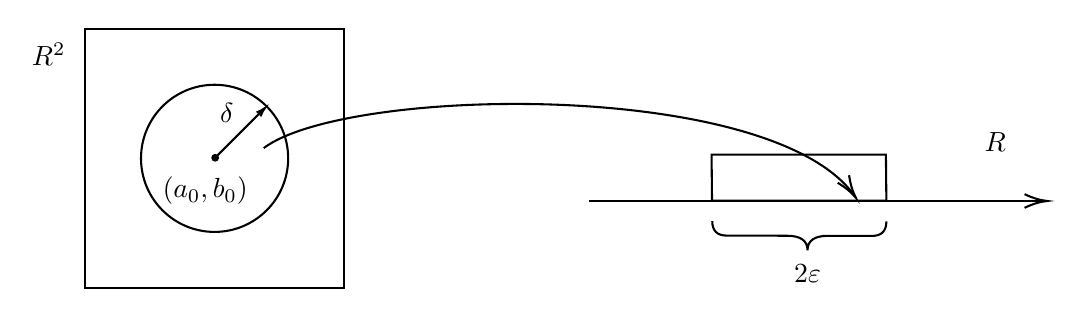
\begin{tikzpicture}[x=0.75pt,y=0.75pt,yscale=-1,xscale=1]
%uncomment if require: \path (0,300); %set diagram left start at 0, and has height of 300

%Shape: Square [id:dp9170661653714376] 
\draw   (119.1,81) -- (244,81) -- (244,205.9) -- (119.1,205.9) -- cycle ;
%Shape: Circle [id:dp10572791246858726] 
\draw   (146.1,143.45) .. controls (146.1,123.87) and (161.97,108) .. (181.55,108) .. controls (201.13,108) and (217,123.87) .. (217,143.45) .. controls (217,163.03) and (201.13,178.9) .. (181.55,178.9) .. controls (161.97,178.9) and (146.1,163.03) .. (146.1,143.45) -- cycle ;
%Straight Lines [id:da844014040371049] 
\draw    (362,164) -- (580.73,164) ;
\draw [shift={(582.73,164)}, rotate = 180] [color={rgb, 255:red, 0; green, 0; blue, 0 }  ][line width=0.75]    (10.93,-3.29) .. controls (6.95,-1.4) and (3.31,-0.3) .. (0,0) .. controls (3.31,0.3) and (6.95,1.4) .. (10.93,3.29)   ;
%Curve Lines [id:da9717239927480394] 
\draw [line width=3] [line join = round][line cap = round]    ;
%Straight Lines [id:da9421804366059203] 
\draw    (181.83,143.18) -- (192.27,132.74) -- (204.42,120.59) ;
\draw [shift={(205.83,119.18)}, rotate = 135] [color={rgb, 255:red, 0; green, 0; blue, 0 }  ][line width=0.75]    (4.37,-1.32) .. controls (2.78,-0.56) and (1.32,-0.12) .. (0,0) .. controls (1.32,0.12) and (2.78,0.56) .. (4.37,1.32)   ;
\draw [shift={(181.83,143.18)}, rotate = 315] [color={rgb, 255:red, 0; green, 0; blue, 0 }  ][fill={rgb, 255:red, 0; green, 0; blue, 0 }  ][line width=0.75]      (0, 0) circle [x radius= 1.34, y radius= 1.34]   ;
%Shape: Polygon [id:ds4718685600955079] 
\draw   (504.99,141.68) -- (505.22,163.84) -- (421.22,163.84) -- (420.99,141.68) -- cycle ;
%Curve Lines [id:da49681144914231967] 
\draw    (205.22,138.51) .. controls (245.02,108.66) and (450.37,105.05) .. (489.97,161.65) ;
\draw [shift={(490.55,162.51)}, rotate = 236.46] [color={rgb, 255:red, 0; green, 0; blue, 0 }  ][line width=0.75]    (10.93,-3.29) .. controls (6.95,-1.4) and (3.31,-0.3) .. (0,0) .. controls (3.31,0.3) and (6.95,1.4) .. (10.93,3.29)   ;
%Shape: Brace [id:dp5810445884123745] 
\draw   (421.33,173.67) .. controls (421.32,178.34) and (423.65,180.67) .. (428.32,180.68) -- (457.23,180.74) .. controls (463.9,180.75) and (467.23,183.09) .. (467.22,187.76) .. controls (467.23,183.09) and (470.56,180.77) .. (477.23,180.78)(474.23,180.78) -- (498.2,180.83) .. controls (502.87,180.84) and (505.21,178.51) .. (505.22,173.84) ;

% Text Node
\draw (92,86.4) node [anchor=north west][inner sep=0.75pt]    {$\mathbb{R}^{2}$};
% Text Node
\draw (182.72,115.57) node [anchor=north west][inner sep=0.75pt]    {$\delta $};
% Text Node
\draw (155.19,151.04) node [anchor=north west][inner sep=0.75pt]  [xslant=0.02]  {$( a_{0} ,b_{0})$};
% Text Node
\draw (459.33,193.4) node [anchor=north west][inner sep=0.75pt]    {$2\varepsilon $};
% Text Node
\draw (551,129.4) node [anchor=north west][inner sep=0.75pt]    {$\mathbb{R}$};


\end{tikzpicture}

\end{proof}

\begin{proposition}
    设$f,g\colon X \to \mathbb{R}$, 定义$F \equiv \left( f\left( x \right) ,g\left( x \right)  \right) $. 
    
    则$F$在$x_0$处连续, 当且仅当$f$和$g$在$x_0$处连续.
\end{proposition}
\begin{proof}
    \textbf{``$\impliedby$''} 设$f,g$在$x_0$处连续, 来证$F$在$x_0$处连续.

    为此$\forall B_{\varepsilon} \left( f\left( x_0 \right) ,g\left( x_0 \right)  \right) $, $\exists \varepsilon' = \frac{\sqrt{2}}{2}\varepsilon$使
    \begin{equation}
      B_{\varepsilon'} \left( f\left( x_0 \right)  \right) \times  B_{\varepsilon'} \left( g\left( x_0 \right)  \right) \subseteq B_{\varepsilon} \left( F\left( x_0 \right) \right).
    \end{equation}

    由$f$在$x_0$处连续, $\exists $ $x_0$的开邻域$U_1$, 使$f\left( U_1 \right) \subseteq  B_{\varepsilon'} \left( f\left( x_0 \right)  \right) $.

    由$g$在$x_0$处连续, $\exists $ $x_0$的开邻域$U_2$使$g\left( U_2 \right) \subseteq B_{\varepsilon'} \left( g\left( x_0 \right)  \right) $.

    取$U = U_1 \cap  U_2$, 则$U$是$x_0$的开邻域, 且
    \begin{equation}
      F\left( U \right) \subseteq f\left( U \right) \times g\left( U \right)  \subseteq f\left( U_1 \right) \times g\left( U_2 \right) \subseteq B_{\varepsilon'} \left( f\left( x_0 \right)  \right) \times B_{\varepsilon'} \left( g\left( x_0 \right)  \right) \subseteq B_{\varepsilon} \left( F\left( x_0 \right)  \right).
    \end{equation}
\end{proof}

\noindent
\textbf{推论: }设$f,g \in C\left( X, \mathbb{R} \right) $则$f+g,\ f-g,\  fg\ \in C\left( X, \mathbb{R} \right) $.

下面来考虑$\frac{f}{g}\left( x \right)  = \frac{f\left( x \right) }{g\left( x \right) }$. 商函数的定义域为$X / g^{-1} \left( \{ 0 \} \right) $.

\begin{proposition}[连续函数的等高面皆为闭集]
    设$f\colon X\to \mathbb{R}$连续, $\forall C \in \mathbb{R}$, 定义
    \begin{equation}
      X_{c} \equiv \{ x\in X | f\left( x \right)  = c \} = f^{-1} \left( \{ c \}  \right) .
    \end{equation}
    则$X_{c}$是闭集.
\end{proposition}
\begin{proof}
    由于单点集$\{ c \}$是$\mathbb{R}$的闭集\footnote{
        只要证$\forall y\neq c$, $\exists  B_{r}\left( y \right) \subseteq \{ c \}^{C}$. 取$r = \frac{1}{2} d\left( y,c \right) > 0$即可.

        同理, $\mathbb{R}^{n}$中单点集也是闭集
    }, 显然.
\end{proof}

\begin{proposition}
    $\forall f \in C\left( X , \mathbb{R}^{n} \right) $, $\forall \vec{c} \in \mathbb{R}^{n}$, 有$f^{-1} \left( \{ \vec{C} \} \right) $是$X$的闭集.
\end{proposition}

\begin{theorem}
    设$f,g \in  C\left( X, \mathbb{R} \right) $连续, 则$\frac{f}{g}$是$X / g^{-1} \left( \{ 0 \} \right) $上的连续映射(即连续函数的商在分母的零点之外连续).
\end{theorem}
\begin{proof}
    令$Y = X / g^{-1}\left( \{ 0 \} \right) $,
    \begin{equation}
      Y \xlongrightarrow{F} \mathbb{R} \times \left( \mathbb{R} / \{ 0 \} \right) \xlongrightarrow{q} \mathbb{R},\quad x \mapsto \left( f\left( x \right) ,g\left( x \right)  \right), \quad q = \frac{f\left( x \right) }{g\left( x \right) }.
    \end{equation}
\end{proof}

\begin{example}
    多项式函数都是连续的.
\end{example}
\begin{proof}
    乘方$x^{n}$是恒同映射的乘法, 是连续的. 加法是连续的.
\end{proof}

\begin{example}
    有理函数在分母的零点之外是连续的.
\end{example}
\begin{proof}
    有理函数是多项式的商函数.
\end{proof}

\begin{proposition}
    设$u\left( x \right) , \ v\left( x \right) $在$x_0$处是连续的, 则$u\left( x \right) ^{v\left( x \right)}$在$x_0$处连续.
\end{proposition}
\begin{proof}[证法一]
    结论等价于 $\displaystyle \lim_{x \to x_0} u\left( x \right) ^{v\left( x \right) } = \left( \lim_{x \to x_0} u\left( x \right)  \right)^{\left( \displaystyle  \lim_{x \to x_0} v\left( x \right)  \right) } $
\end{proof}
\begin{proof}[证法二]
    $u\left( x \right) ^{v\left( x \right) } = \mathrm{e}^{v\left( x \right) \ln u\left( x \right) }$.

    $u\left( x \right) $与$\ln(\square)$复合, 再与乘法复合, 再与$\mathrm{e}^{(\square)}$复合
\end{proof}